
\documentclass{tufte-handout}

%\geometry{showframe}% for debugging purposes -- displays the margins
\usepackage{setspace}
\usepackage{pdfpages}
\usepackage{ifthen}
\usepackage{amsthm}
\usepackage{enumitem}
\usepackage{kpfonts}
\newcommand*{\vv}[1]{\vec{\mkern0mu#1}}

\usepackage{graphicx}
\setkeys{Gin}{width=\linewidth,totalheight=\textheight,keepaspectratio}
\graphicspath{{graphics/}}
\usepackage{xcolor}
\title{iQ3R Mathematics --- Geometry\thanks{Typically in the United States grade 9 students take either Algebra 1 or Geometry depending on the school and the performance of the student in 8th grade. Generally, Geometry is taken by students who are on a more accelerated track.} \\ 
Lesson 6 Module 1 \thanks{Adapted for individualized instruction from the EngageNY curriculum for New York State public and private instructors.}}
%\author[The Tufte-LaTeX Developers]{Instructor Version\footnote{Instructor notes will appear along the side column.}}  % if the \date{} command is left out, the current date will be used
\usepackage{pgf,pgfplots,tikz}
%\pgfplotset{compat=1.5}
\usetikzlibrary{calc,through,backgrounds,arrows}
\usepackage[most]{tcolorbox}
\usepackage{tikzsymbols}
\usepackage{tkz-euclide}
\usetkzobj{all}
\usepackage{booktabs}
\usepackage{palatino}
\usepackage{units}
\usepackage{fancyvrb}
\fvset{fontsize=\normalsize}
\usepackage{multicol}
\usepackage{lipsum}
\usepackage[utf8]{inputenc}
% These commands are used to pretty-print LaTeX commands
\newcommand{\doccmd}[1]{\texttt{\textbackslash#1}}% command name -- adds backslash automatically
\newcommand{\docopt}[1]{\ensuremath{\langle}\textrm{\textit{#1}}\ensuremath{\rangle}}% optional command argument
\newcommand{\docarg}[1]{\textrm{\textit{#1}}}% (required) command argument
\newenvironment{docspec}{\begin{quote}\noindent}{\end{quote}}% command specification environment
\newcommand{\docenv}[1]{\textsf{#1}}% environment name
\newcommand{\docpkg}[1]{\texttt{#1}}% package name
\newcommand{\doccls}[1]{\texttt{#1}}% document class name
\newcommand{\docclsopt}[1]{\texttt{#1}}% document class option name
\newcommand{\n}{\noindent}
\newcommand{\uv}{\vspace{.1in}}
\newcommand{\uvx}{\vspace{.2in}}
\newcommand{\uvxx}{\vspace{.3in}}
\newtheorem{myex}{Example}
\newtheorem{mythm}{Theorem}
\newtheorem{mydef}{Definition}
\newtheorem{myprob}{Problem}
\newtheorem{note}{Note}
\newtheorem{prac}{Guided Practice}
\newtheorem{ex}{Exercise}
\begin{document}
\definecolor{wrwrwr}{rgb}{0.3803921568627451,0.3803921568627451,0.3803921568627451}
\definecolor{rvwvcq}{rgb}{0.08235294117647059,0.396078431372549,0.7529411764705882}
\definecolor{dtsfsf}{rgb}{0.8274509803921568,0.1843137254901961,0.1843137254901961}
\definecolor{rvwvcq}{rgb}{0.08235294117647059,0.396078431372549,0.7529411764705882}
 \maketitle
 
 \begin{abstract}
     This sixth lesson is a bit of a departure from the New York curriculum. Instead of starting into Topic B, we find it best to review the material in Topic A and to tie together some concepts we left unaddressed in Topic A. Students will still practice using the construction tools and techniques introduced in lessons 1 through 5, but here we will close the gaps in some of the reasoning that was used to assert some of the claims made in those lessons. \end{abstract}
     
  %Slide  1 xxxxxxxxxxxxxxxxxxxxxxxxxxxxxxxxxxxxxxxxxxxxxxxxxxxxxxxxxxxxxxxxxxxx
\marginnote[]{\section{Overview}\subsection{Lesson 6 Supported Standards}
\begin{tcolorbox}[enhanced jigsaw,breakable,pad at break*=1mm,
  colback=cyan!5!white,colframe=red!75!black,title= Common Core Focus Standards, drop fuzzy shadow,
  watermark color=white,watermark text=\arabic{tcbbreakpart}]
 \textbf{G-CO.A.1} \\
 Know precise definitions of angle, circle, perpendicular line, parallel line, and line segment, based on the undefined notions of point, line, distance along a line, and distance around a circular arc.
 
 \vspace{.1in}
 \textbf{G-CO.D.12} \\
 Make formal geometric constructions with a variety of tools and methods (compass and
straightedge, string, reflective devices, paper folding, dynamic geometric software,
etc.). Copying a segment; copying an angle; bisecting a segment; bisecting an angle;
constructing perpendicular lines, including the perpendicular bisector of a line segment;
and constructing a line parallel to a given line through a point not on the line.

\vspace{.1in}
\textbf{G-CO.D.13} \\
Construct an equilateral triangle, a square, and a regular hexagon inscribed in a circle.
   \end{tcolorbox}}


\begin{tcolorbox}[enhanced jigsaw,breakable,pad at break*=1mm,
  colback=cyan!2!white,colframe=blue!75!black,title=Student View: Slide 1,drop fuzzy shadow,watermark color=white,watermark text=\arabic{tcbbreakpart}]
  \section{Overview}
  \newthought{In this lesson} you will bring together all the ideas you learned in lessons 1 through 5. This will complete this unit on constructions. Specifically the aim of this lesson is to 
  \begin{enumerate}
      \item Review basic constructions: you will also learn to find perpendiculars through points on lines; parallels through points not on lines. 
      \item Discuss postulates vs. assumptions. 
      \item Introduce measurement concepts: how to measure distance between various geometric objects.
      \item Introduce you to symmetry. 
      \item Help you see ``why'' the concurrences we saw in lessons 4 and 5 occur.
  \end{enumerate}
  
 
\end{tcolorbox}
%End Slide   1 xxxxxxxxxxxxxxxxxxxxxxxxxxxxxxxxxxxxxxxxxxxxxxxxxxxxxxxxxxxxxxxxx

\pagebreak

%Slide  2 xxxxxxxxxxxxxxxxxxxxxxxxxxxxxxxxxxxxxxxxxxxxxxxxxxxxxxxxxxxxxxxxxxxx
\marginnote[]{\section{Review with Applications}\subsection{Basic Constructions}
\begin{enumerate}
    \item Students have seen these procedures and have been using them over the last five lessons so the procedures will not be reproduced here. Be prepared to verbally review them if necessary. 
    \begin{tcolorbox}[colback=yellow]
      Do we want to have some form of digital handout they can reference?
    \end{tcolorbox}
\end{enumerate}

}
\begin{tcolorbox}[enhanced jigsaw,breakable,pad at break*=1mm,
  colback=cyan!2!white,colframe=blue!75!black,title=Student View: Slide 2,drop fuzzy shadow,watermark color=white,watermark text=\arabic{tcbbreakpart}]
 \section{Review with Applications}\subsection{Basic Constructions}
 You now know$^1$ three basic constructions using the drawing tools
 \begin{itemize}
     \item Given a line segment, find the perpendicular bisector to the line segment.
     \item Given an angle, find the angle bisector of that angle.
     \item Given an angle, copy the angle along another segment or ray.
 \end{itemize}
 
 Using these basic constructions, you now are able to 
 \begin{itemize}
     \item Construct an equilateral triangle
     \item Construct a regular hexagon
     \item Find the perpindicular to a given line which contains a specified point not on the line.
     \item Construct the incenter and circumcenter of a triangle as well as the corresponding circles.
 \end{itemize}

\newthought{Check For Understanding:} Given a triangle $\triangle ABC$ draw
\begin{enumerate}
    \item The circumcircle
    \item The incircle
\end{enumerate}
\newthought{Challenge:} When will the circumcenter of a triangle be on the exterior of the triangle? When will it be on one of the sides of a triangle? 
\end{tcolorbox}
%End Slide 2 xxxxxxxxxxxxxxxxxxxxxxxxxxxxxxxxxxxxxxxxxxxxxxxxxxxxxxxxxxxxxxxxx


\pagebreak
\marginnote[.5in]{
\begin{enumerate}
    \item Ask, ``Do we really need to find all three perpendicular bisectors to draw the circumcircle?''
    \item Note that we have not included \textbf{\textit{arrowheads}} in the picture. When the line extends to the border of the graphic, that also is intended to represent a line. When we want to emphasize that a portion of a line is being viewed, we will do that by keeping the entire structure within the viewing window and useing the arrowheads where the segment terminates.
\end{enumerate}

}

\begin{tcolorbox}[enhanced jigsaw,breakable,pad at break*=1mm,attach boxed title to top center={yshift=-3mm,yshifttext=-1mm},
  colback=yellow!50!white,colframe=yellow,colbacktitle=red!80!black,
  title=Lesson Design Specifications (Please Read),fonttitle=\bfseries,
  boxed title style={size=small,colframe=red!50!black} ]
  \section{Guided Practice: }
 At this point student and teacher will do one of the following: 
    \begin{itemize}
      \item Navigate to Geogebra on a shared screen \textbf{OR}
      \item Launch an app that opens up a shared window for interactive geometry \textbf{OR}
      \item Share a whiteboard with appropriate drawing tools.
  \end{itemize}
Instructor will now use the following sequence on first a scalene then an obtuse triangle. We show only the case for the obtuse. 

 \newthought{Construction Sequence}
 
 \uv
  \begin{minipage}{0.5\textwidth}
\scalebox{1}{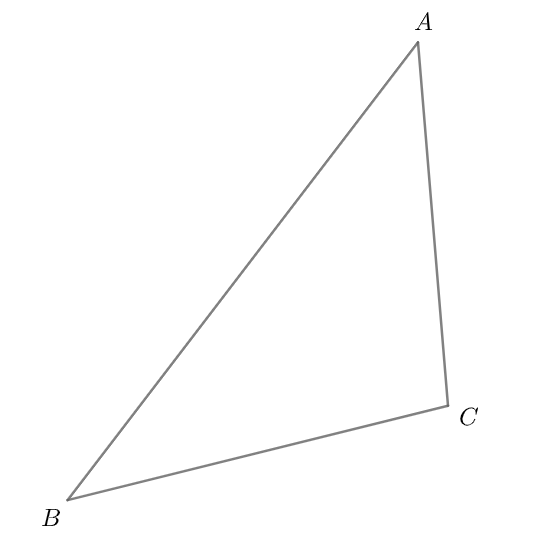
\includegraphics[]{circmcent0.png}}
\end{minipage} \hfill
\begin{minipage}{0.45\textwidth}
\setstretch{.7}
\begin{scriptsize}
\newthought{Step 1}

\uv
Find the perpendicular bisectors of the segments of $\triangle ABC.$ Label their point of concurrency$^1$ $J.$
\end{scriptsize}
\end{minipage}

 \uv
  \begin{minipage}{0.5\textwidth}
\scalebox{1}{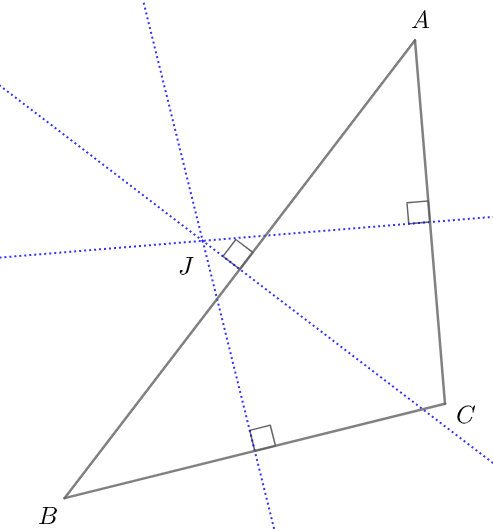
\includegraphics[]{circmcent1.png}}
\end{minipage} \hfill
\begin{minipage}{0.45\textwidth}
\setstretch{.7}
\begin{scriptsize}
\newthought{Step 2}

\uv
The result should look something like the figure shown$^2$. Ask, ``What radius should you use for the circle centered at $J$?'' \textbf{\textit{Answer:}} Any of the equal distances $AJ, \ BJ$ or $CJ$ will do.

\uv Now draw circle $J$ with the appropriate radius. 
\end{scriptsize}
\end{minipage}
\end{tcolorbox}

\pagebreak
\begin{tcolorbox}[enhanced jigsaw,breakable,pad at break*=1mm,attach boxed title to top center={yshift=-3mm,yshifttext=-1mm},
  colback=yellow!50!white,colframe=yellow,colbacktitle=red!80!black,
  title=Lesson Design Specifications (Please Read),fonttitle=\bfseries,
  boxed title style={size=small,colframe=red!50!black} ]
  \section{Guided Practice: Continued }
  \begin{minipage}{0.5\textwidth}
\scalebox{1}{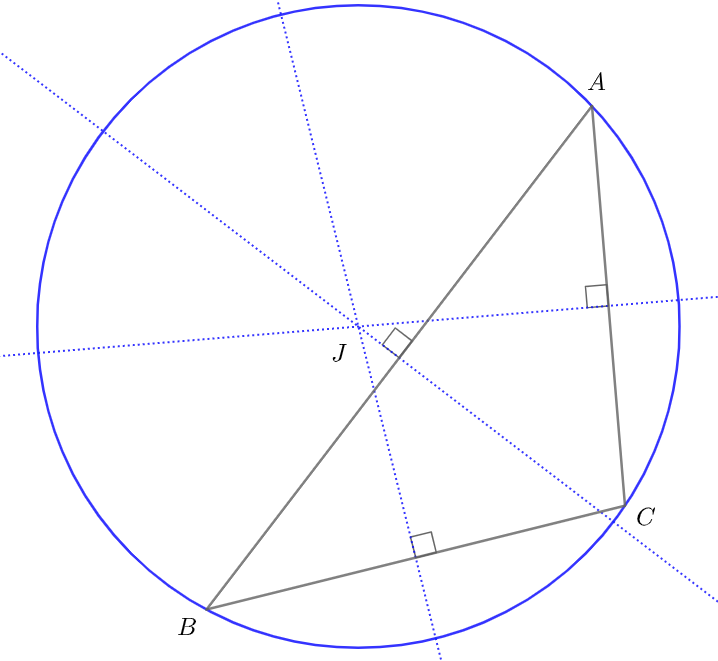
\includegraphics[]{circmcent2.png}}
\end{minipage} \hfill
\begin{minipage}{0.45\textwidth}
\setstretch{.7}
\begin{scriptsize}
\newthought{Step 3}

\uv
The result should look something like the figure shown. Now clear away the auxillary lines and miscellaneous label $J.$ 

\uv Leave the circum-circle in view.


\end{scriptsize}
\end{minipage}

\uvx
\begin{minipage}{0.5\textwidth}
\scalebox{1}{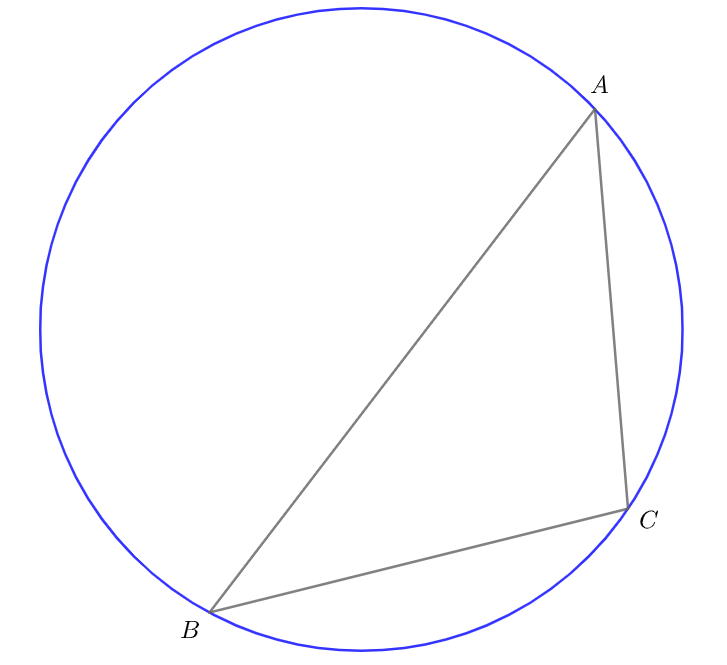
\includegraphics[]{setfornextstage.png}}
\end{minipage} \hfill
\begin{minipage}{0.45\textwidth}
\setstretch{.7}
\begin{scriptsize}
\newthought{Step 4}

\uv
Now draw the bisectors of each of the angles of triangle $\triangle ABC.$ 

\uv Label the incenter as $K$.


\end{scriptsize}
\end{minipage}

\uvx
\begin{minipage}{0.5\textwidth}
\scalebox{1}{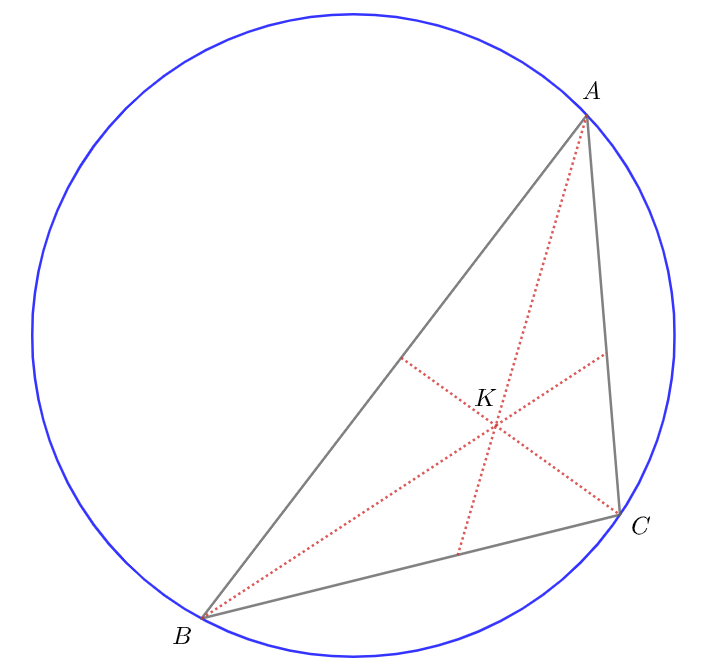
\includegraphics[]{incir1.png}}
\end{minipage} \hfill
\begin{minipage}{0.45\textwidth}
\setstretch{.7}
\begin{scriptsize}
\newthought{Step 5}

\uv
The result should appear somewhat like what you see here in this figure.

\uv Next, draw a perpendicular segment from $K$ to side $BC$ and label its intersection with $BC$ as $L.$


\end{scriptsize}
\end{minipage}
\end{tcolorbox}
\pagebreak

\begin{tcolorbox}[enhanced jigsaw,breakable,pad at break*=1mm,attach boxed title to top center={yshift=-3mm,yshifttext=-1mm},
  colback=yellow!50!white,colframe=yellow,colbacktitle=red!80!black,
  title=Lesson Design Specifications (Please Read),fonttitle=\bfseries,
  boxed title style={size=small,colframe=red!50!black} ]
  \section{Guided Practice: Continued}
\begin{minipage}{0.5\textwidth}
\scalebox{1}{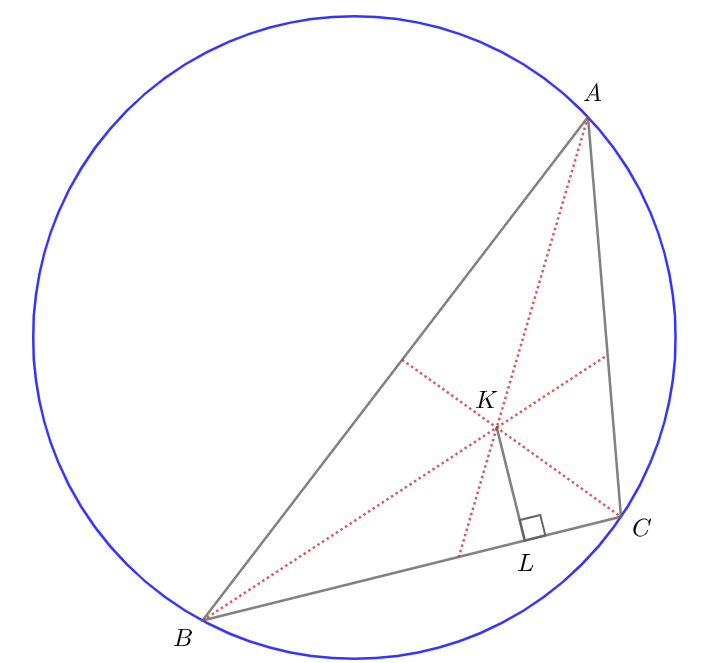
\includegraphics[]{incir2.png}}
\end{minipage} \hfill
\begin{minipage}{0.45\textwidth}
\setstretch{.7}
\begin{scriptsize}
\newthought{Step 6}

\uv
The result should appear somewhat like what you see here in this figure. 

\uv Finally, draw circle $K$ centered at $K$ with radius $KL.$




\end{scriptsize}
\end{minipage}

\uvx
\begin{minipage}{0.5\textwidth}
\scalebox{1}{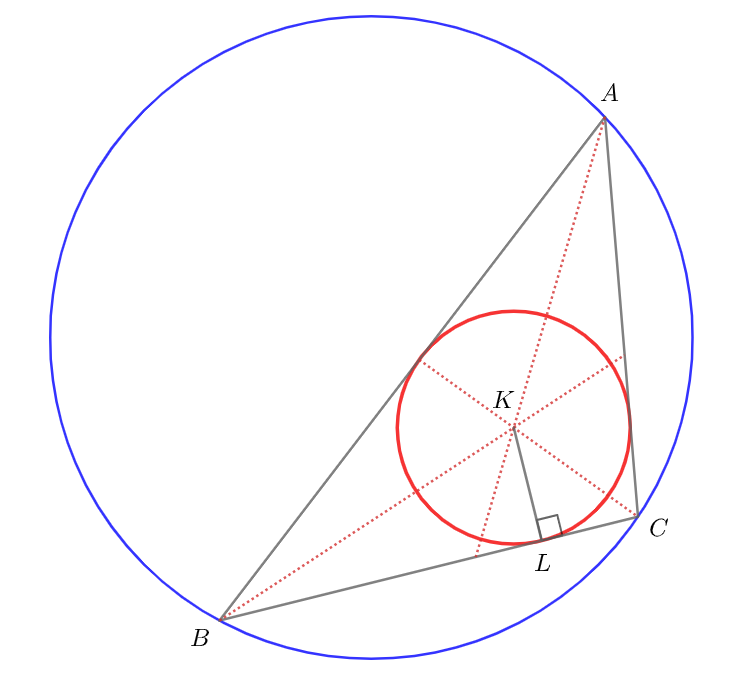
\includegraphics[]{incir3.png}}
\end{minipage} \hfill
\begin{minipage}{0.45\textwidth}
\setstretch{.7}
\begin{scriptsize}
\newthought{Step 7}

\uv
The result should appear somewhat like what you see here in this figure. 

\uv Now eliminate all the superflous lines and labels. 




\end{scriptsize}
\end{minipage}

\uvx
\begin{minipage}{0.5\textwidth}
\scalebox{1}{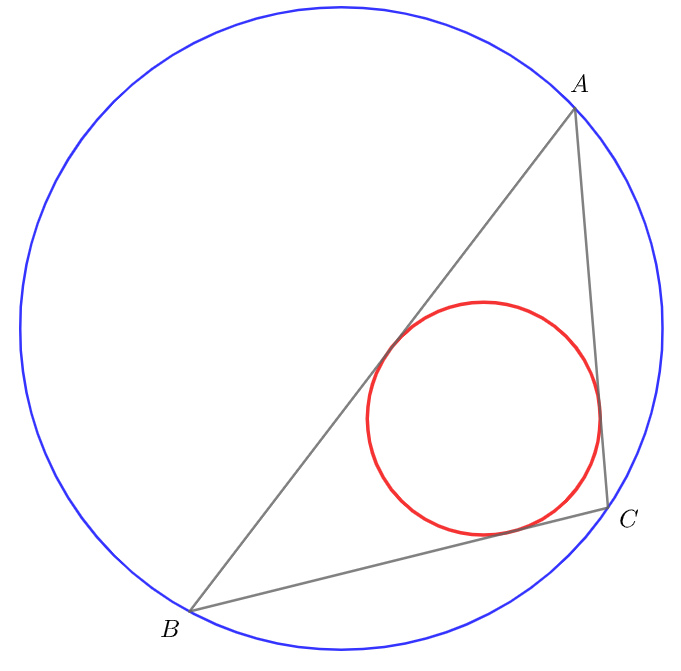
\includegraphics[]{incir4.png}}
\end{minipage} \hfill
\begin{minipage}{0.45\textwidth}
\setstretch{.7}
\begin{scriptsize}
The final figure with a triangle showing BOTH the incircle and the circumcircle. 




\end{scriptsize}
\end{minipage}

\uvxx

Now we return to the main instructional sequence. 
\end{tcolorbox}

\pagebreak 
%Slide  3 xxxxxxxxxxxxxxxxxxxxxxxxxxxxxxxxxxxxxxxxxxxxxxxxxxxxxxxxxxxxxxxxxxxx
\marginnote[]{\section{Review with Applications}\subsection{Extending the Results}
\begin{enumerate}
    \item The function notation is intentional. For each line $k$ in the plane $k^{\perp}$ defines a function from the set of points in the plane to the set of lines in the plane. This function has interesting properties on its own.
\end{enumerate}

}
\begin{tcolorbox}[enhanced jigsaw,breakable,pad at break*=1mm,
  colback=cyan!2!white,colframe=blue!75!black,title=Student View: Slide 3,drop fuzzy shadow,watermark color=white,watermark text=\arabic{tcbbreakpart}]
  \section{Review with Applications}\subsection{Extending the Results}
  Previously: For given line $k$ and point $P$ not on $k$ we saw how to use our basic constructions to find the line perpendicular to $k$ through $P.$ We now make a definition/notation which we will stay with for the course.
  
  \uv \newthought{Definition $k^{\perp}(P)$:} Given line $k$ and point $P$ (either on or off of $k$), we represent \textbf{\textit{the unique}} line which is perpendicular to $k$ and contains $P$ by the notation$^1$ $k^{\perp}(P).$ 
  
  \uv \newthought{Definition $k^{\parallel}(P):$} Given a line $k$ and a point $P$ (again, either on or off of $k$), we represent the unique line which is parallel to $k$ through $P$ by the notation $k^{\parallel}(P).$ If a point $P$ is on $k$ we take $k^{\parallel}(P)$ to simply be $k.$
  
  
  \newthought{Knowledge Point:} Using the basic constructions you now can
  \begin{enumerate}
      \item Construct $k^{\perp}(P)$, given line $k$ and point $P$ in any case --- whether $P$ is on $k$ or not.
      \item Construct $k^{\parallel}(P)$ for any given line $k$ and point $P$. 
  \end{enumerate}
  Let's work out the details of (1) first.
 
\end{tcolorbox}
%End Slide  3 xxxxxxxxxxxxxxxxxxxxxxxxxxxxxxxxxxxxxxxxxxxxxxxxxxxxxxxxxxxxxxxxx

\pagebreak

\begin{tcolorbox}[enhanced jigsaw,breakable,pad at break*=1mm,attach boxed title to top center={yshift=-3mm,yshifttext=-1mm},
  colback=yellow!50!white,colframe=yellow,colbacktitle=red!80!black,
  title=Lesson Design Specifications (Please Read),fonttitle=\bfseries,
  boxed title style={size=small,colframe=red!50!black} ]
  \section{Guided Practice 2: Construction of $k^{\perp}(P)$; case $P$ is on $k.$ }
 At this point student and teacher will do one of the following: 
    \begin{itemize}
      \item Navigate to Geogebra on a shared screen \textbf{OR}
      \item Launch an app that opens up a shared window for interactive geometry \textbf{OR}
      \item Share a whiteboard with appropriate drawing tools.
  \end{itemize}
  
  \uvx
  
  \begin{minipage}{0.65\textwidth}
\scalebox{1}{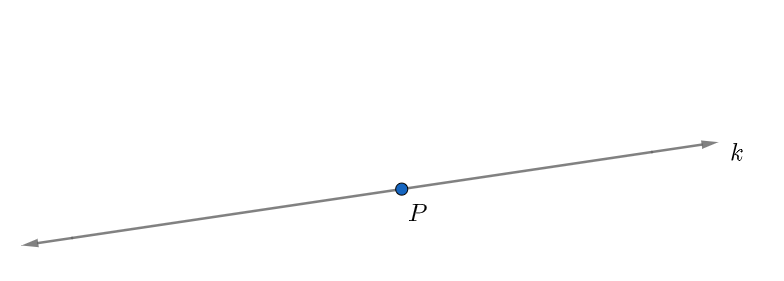
\includegraphics[]{thruP1.png}}
\end{minipage} \hfill
\begin{minipage}{0.32\textwidth}
\setstretch{.7}
\begin{scriptsize}
\newthought{\textbf{Step 1:}} Fix line $k$ with selection of arbitrary point $P$ on $k.$
 Draw a circle with center at $P$ and label intersections as $A$ and $B.$
 \end{scriptsize}
\end{minipage}

\uvx
  \begin{minipage}{0.65\textwidth}
\scalebox{1}{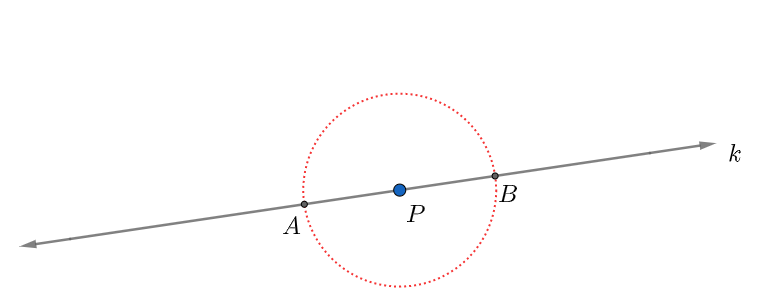
\includegraphics[]{thruP2.png}}
\end{minipage} \hfill
\begin{minipage}{0.32\textwidth}
\setstretch{.7}
\begin{scriptsize}
\newthought{\textbf{Step 2:}} Now find $\mathcal{L}_{AB}^{\perp}$ --- the perpendicular bisector of segment $AB.$
 \end{scriptsize}
\end{minipage}


\uvx
  \begin{minipage}{0.65\textwidth}
\scalebox{1}{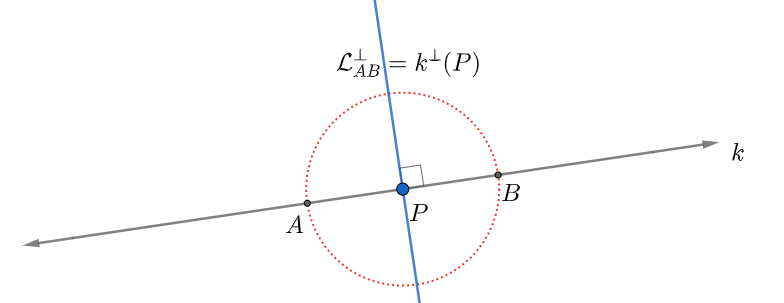
\includegraphics[]{thruP3.png}}
\end{minipage} \hfill
\begin{minipage}{0.32\textwidth}
\setstretch{.7}
\begin{scriptsize}

\newthought{\textbf{Step 3:}} Done. We have done what we set out to do. We have found $k^{\perp}(P)$ --- the line perpendicular to $k$ through the point $P$ \textbf{\textit{located on}} $k.$


 \end{scriptsize} 
\end{minipage}

\uvxx
We now return to the main sequence of instructional slides.
\end{tcolorbox}

\pagebreak

%Slide  4 xxxxxxxxxxxxxxxxxxxxxxxxxxxxxxxxxxxxxxxxxxxxxxxxxxxxxxxxxxxxxxxxxxxx
\marginnote[]{\section{Review with Applications}\subsection{Construction of $k{\perp}(P).$}


}
\begin{tcolorbox}[enhanced jigsaw,breakable,pad at break*=1mm,
  colback=cyan!2!white,colframe=blue!75!black,title=Student View: Slide 4,drop fuzzy shadow,watermark color=white,watermark text=\arabic{tcbbreakpart}]
  \section{Review with Applications}\subsection{Construction of $k^{\perp}(P).$}
  \newthought{Notation:} If a line $k$ is specified with selected point $P$ on $k$, we will represent the line perpendicular to $k$ containing the point $P$ by the symbol $k^{\perp}(P)$ --- pronounced ``k perp of P''. 
  
  \newthought{Knowledge Point:} Construction of $k^{\perp}(P)$ from line $k$ and point $P$ on line $k.$
  \begin{itemize}
      \item Step 1: Locate $P$ on line $k$.
      \item Step 2: Draw circle $P$ centered at $P$ with any positive radius $r.$ Since $r>0$ circle $P$ meets $k$ in exactly two points which we label $A$ and $B.$
      \item Step 3: Draw $\mathcal{L}_{AB}^{\perp}$ --- the perpendicular bisector of segment $AB.$ 
      \item Observation: $\mathcal{L}_{AB}^{\perp}= k^{\perp}(P)$.
  \end{itemize}
  
  \uvx We now address the second problem we considered.
  
 
\end{tcolorbox}
%End Slide   4xxxxxxxxxxxxxxxxxxxxxxxxxxxxxxxxxxxxxxxxxxxxxxxxxxxxxxxxxxxxxxxxx

\pagebreak
%Slide   5xxxxxxxxxxxxxxxxxxxxxxxxxxxxxxxxxxxxxxxxxxxxxxxxxxxxxxxxxxxxxxxxxxxx
\marginnote[]{\section{Review with Applications}\subsection{Construction of $k_{||}^P$}
\begin{enumerate}
    \item Be sure to emphasize that the words go with the symbol. When they see the symbol $k^{\parallel}(P)$ they should be thinking ``the line parallel to line $k$ through the point $P$.'' We use the symbol so we don't have to keep writing the cumbersome phrase over and over again, but we MUST remember that the symbol is encoding the language of geometry. 
    \item We mean the arrows around the ``center'' of the figure. Recall our convention: lines are either represented as in the figure by $k$ using arrows on the ends of the segment, or as in the figure by $k^{\parallel}(P)$ which simply runs from one side of the viewing window to the other. 
\end{enumerate}

}
\begin{tcolorbox}[enhanced jigsaw,breakable,pad at break*=1mm,
  colback=cyan!2!white,colframe=blue!75!black,title=Student View: Slide 5,drop fuzzy shadow,watermark color=white,watermark text=\arabic{tcbbreakpart}]
 \section{Review with Applications}\subsection{Construction of $k^{\parallel}(P)$}
 \newthought{Important Problem:} Given line $k$ and point $P$, off $k$, find a line which is both parallel to $k$ and contains $P$. Recall that we use the notation$^1$ $k^{\parallel}(P)$ to represent this line: \textbf{\textit{The}} line \textbf{\textit{parallel}} to line $k$ containing the point $P$ which is off $k$. This is illustrated in the figure below.
 
 \begin{center}
 \scalebox{1}{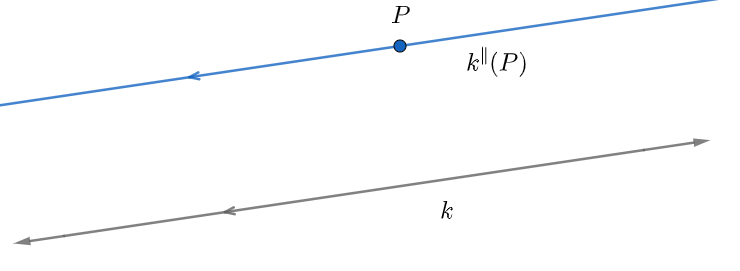
\includegraphics[]{para0.png}}
 \end{center}
 
 We use the arrows$^2$ along the lines for emphasis that these lines are parallel. 
 
 \uv Let's see how this construction works \dCooley[-2][yellow]
 
 
  
 
\end{tcolorbox}
%End Slide  5 xxxxxxxxxxxxxxxxxxxxxxxxxxxxxxxxxxxxxxxxxxxxxxxxxxxxxxxxxxxxxxxxx
\pagebreak

\marginnote[.5in]{
\begin{enumerate}
    \item What would happen if we tried to pick point $P$ on line $k$?
    \item Again, stress that what you label the lines and points does not matter. Notice that when we label lines other than by using notation like $\overleftrightarrow{AB}$, we use either lower case letters or the more elaborate $\mathcal{L}$.
    \item QED --- \textbf{\textit{quod erat demonstrandum}} --- Latin for ``what was to be demonstrated''
\end{enumerate}

}

\begin{tcolorbox}[enhanced jigsaw,breakable,pad at break*=1mm,attach boxed title to top center={yshift=-3mm,yshifttext=-1mm},
  colback=yellow!50!white,colframe=yellow,colbacktitle=red!80!black,
  title=Lesson Design Specifications (Please Read),fonttitle=\bfseries,
  boxed title style={size=small,colframe=red!50!black} ]
  \section{Guided Practice: }
 At this point student and teacher will do one of the following: 
    \begin{itemize}
      \item Navigate to Geogebra on a shared screen \textbf{OR}
      \item Launch an app that opens up a shared window for interactive geometry \textbf{OR}
      \item Share a whiteboard with appropriate drawing tools.
  \end{itemize}
  
  Instructor will now guide the student through the steps required to construct $k^{\parallel}(P)$.
  
\uv
  
\begin{minipage}{0.65\textwidth}
\scalebox{1}{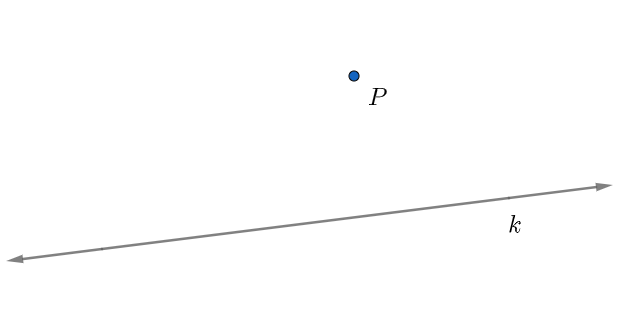
\includegraphics[]{para1.png}}
\end{minipage} \hfill
\begin{minipage}{0.32\textwidth}
\setstretch{.7}
\begin{scriptsize}
\newthought{\textbf{Step 1:}}
Start with a given line $k$ and point not$^1$ on $k$  which we have labeled $P.$ $^2$ Using the ideas from lesson 4, construct the perpendicular to $k$ containing point $P$. Call this $q$. (Observe that $q=k^{\perp}(P).$)
\end{scriptsize} 
\end{minipage}

\uv
  
\begin{minipage}{0.65\textwidth}
\scalebox{1}{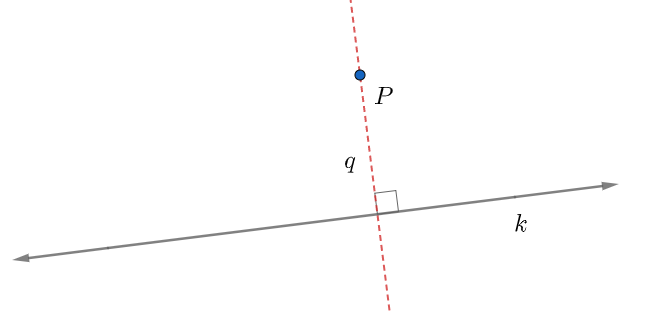
\includegraphics[]{para2.png}}
\end{minipage} \hfill
\begin{minipage}{0.32\textwidth}
\setstretch{.7}
\begin{scriptsize}
\newthought{\textbf{Step 2:}}
You should get a figure similar to the one shown here at the left. Now have the student construct $q^{\perp}(P)$ --- the line perpendicular to $q$ through $P.$
\end{scriptsize} 
\end{minipage}

\uv
  
\begin{minipage}{0.65\textwidth}
\scalebox{1}{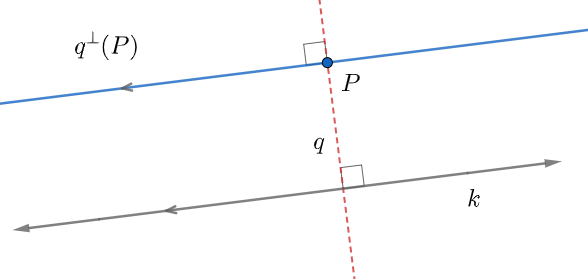
\includegraphics[]{para3.png}}
\end{minipage} \hfill
\begin{minipage}{0.32\textwidth}
\setstretch{.7}
\begin{scriptsize}
\newthought{\textbf{Step 3:}}
That is it! Amazing! Acutually $q^{\perp}(P)$ is what you are looking for. We emphasize this in the next figure.
\end{scriptsize} 
\end{minipage}

\uv
  
\begin{minipage}{0.65\textwidth}
\scalebox{1}{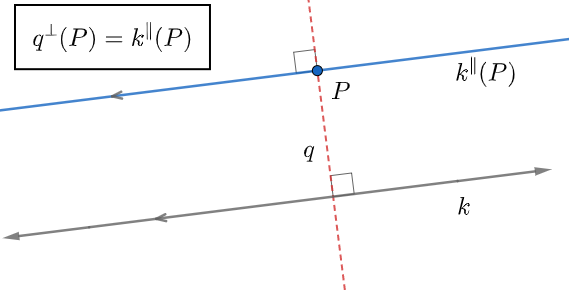
\includegraphics[]{para4.png}}
\end{minipage} \hfill
\begin{minipage}{0.32\textwidth}
\setstretch{.7}
\begin{scriptsize}
\newthought{\textbf{All done! QED$^3$}}
\dCooley[2][cyan]
\end{scriptsize} 
\end{minipage}
\end{tcolorbox}

\pagebreak

%Slide  6 xxxxxxxxxxxxxxxxxxxxxxxxxxxxxxxxxxxxxxxxxxxxxxxxxxxxxxxxxxxxxxxxxxxx
\marginnote[]{\section{Review with Applications}\subsection{Construction of $k^{\parallel}(P)$}
 \begin{enumerate}
    \item Recall that if $P$ is on $K$ then $k^{\parallel}(P)$ is just $k.$
     \item This is truly an instance of where the choice of effective notation really does convey more information than expected. The language here that goes with this little equation is, ``The perp \textbf{\textit{through}} $P$ on the perp \textbf{\textit{from $P$ to $k$}} is the \textbf{\textit{parallel}} to $k$ through $P.$
     \item Focus on the language. The expression says ``find the perpendicular through $P$, to the line \textbf{\textit{parallell to $k$}} which contains $P.$ This must be the perpendicular through $P$ to $k.$ So the answer is simply $k^{\perp}(P).$
 \end{enumerate}

}
\begin{tcolorbox}[enhanced jigsaw,breakable,pad at break*=1mm,
  colback=cyan!2!white,colframe=blue!75!black,title=Student View: Slide 6,drop fuzzy shadow,watermark color=white,watermark text=\arabic{tcbbreakpart}]
  \section{Review with Applications}\subsection{Construction of $k^{\parallel}(P)$}
  
  
  \newthought{Knowledge Point:} If a line $k$ and a point $P$ not on$^1$ $k$ are specified, then we use the following procedure to find $k^{\parallel}(P)$ --- the line parallel to $k$ through the point $P.$
  \begin{itemize}
      \item Step 1: Draw line $k^{\perp}(P)$ containing point $P$.
      \item Step 2: Draw the perpendicular through $P$ to line $k^{\perp}(P)$.
      \item Step 3: Verify that in fact the following beautiful equation$^2$ holds! \[k^{\parallel}(P) = (k^{\perp}(P))^{\perp}(P)\] 
  \end{itemize}
  
  \newthought{Observation:} This equation of line descriptors is an extremely concise way of saying that,``Two lines perpendicular to the same line are parallel to each other."
  
  \newthought{Check For Understanding:} Using our notation$^3$, what should be the result of finding $(k^{\parallel}(P))^{\perp}(P)$?
  
 
\end{tcolorbox}
%End Slide 6  xxxxxxxxxxxxxxxxxxxxxxxxxxxxxxxxxxxxxxxxxxxxxxxxxxxxxxxxxxxxxxxxx

\pagebreak
%Slide  7 xxxxxxxxxxxxxxxxxxxxxxxxxxxxxxxxxxxxxxxxxxxxxxxxxxxxxxxxxxxxxxxxxxxx
\marginnote[]{\section{Concept Development}\subsection{Postulates}
\begin{enumerate}
    \item Postulates are the foundation of the theory of geometry. We can change the parallel postulate to read that there are infinitely many lines parallel to $k.$ When we do that we change from ``flat '' geometry to non-Euclidean geometry. 
    \item It is not a necessary condition of the assumptions of Euclidean Geometry. This is in fact the starting point for non-Euclidean geometries. For centuries, mathematicians tried to ``prove'' the parallel postulate as a consequence of other assumed ``facts'' and were miserably thwarted. Now we know that this postulate is actually what characterizes the Euclidean ``flat'' space.
    \item The physical universe is generally considered to be a 4-dimensional space-time manifold that is ``curved'' due to the presence of matter which is equivalent to gravity according to Einstein. 
\end{enumerate}

}
\begin{tcolorbox}[enhanced jigsaw,breakable,pad at break*=1mm,
  colback=cyan!2!white,colframe=blue!75!black,title=Student View: Slide 7,drop fuzzy shadow,watermark color=white,watermark text=\arabic{tcbbreakpart}]
  \section{Concept Development}\subsection{Postulates}
  \begin{tcolorbox}[colback=blue!4]
  \textbf{\textit{Parallel Postulate:}}
  
  Given a point $P$ and line $k$ not containing $P$ there exists \textbf{\textit{exactly one}} line containing $P$ which is parallel to $k.$
    
  \end{tcolorbox}
  
  Assumptions in Geometry are actually called ``postulates''. 
  
  \begin{itemize}
      \item An assumption can be easily changed.
      \item A postulate$^1$ is something that is taken to be true and is not easily changed.
      \item This ``parallel postulate'' changed the world of geometry!
      \item Since it is an assumption and not a ``fact'', people wondered if it was a necessary condition$^2$ of the assumed ``Euclidean Assumptions.''
      \item This postulate actually characterizes what we call ``flat space'' and it is not necessarily true for all ``spaces.''$^3$
      
  \end{itemize}
  
  
  
 
\end{tcolorbox}

%End Slide7 xxxxxxxxxxxxxxxxxxxxxxxxxxxxxxxxxxxxxxxxxxxxxxxxxxxxxxxxxxxxxxxxx
\pagebreak
%Slide  8 xxxxxxxxxxxxxxxxxxxxxxxxxxxxxxxxxxxxxxxxxxxxxxxxxxxxxxxxxxxxxxxxxxxx



\marginnote[]{\section{Concept Development}\subsection{Postulates}
\begin{enumerate}
    \item For example, it could be units of time, money, length and so on. The idea is that scalars are not just numbers when it comes to measurement in geometry. We measure lengths, or intervals, in units in some fixed system. Be sure to emphasize this. In geometry when we say, for example $AB=2,$ we most always mean $2$ of ``something'' --- unless you are working in a highly specialized dimensionless framework which is way beyond the scope of this course.
    \item One-to-one means that if $x(A)=x(B),$ then $A=B.$ The mapping is also surjective (onto). This is the content of the second part of the postulate.
    \item This is the Greek letter ``zeta''.
    \item Curvelinear coordinate systems are also possible: a standard coordinate system on the ``postive'' axis is given by $x=\log t.$ This is the system in which earthquake magnitudes are measured. 
\end{enumerate}

}
\begin{tcolorbox}[enhanced jigsaw,breakable,pad at break*=1mm,
  colback=cyan!2!white,colframe=blue!75!black,title=Student View: Slide 8,drop fuzzy shadow,watermark color=white,watermark text=\arabic{tcbbreakpart}]\section{Concept Development}\subsection{Postulates}
  
  \begin{tcolorbox}[colback=blue!4]
  \textbf{\textit{The Ruler Postulate:}}
  
  Let point $O$ and $P$ be chosen on line $k.$ Let the real number system, $\mathbb{R,}$ represent measurements in a fixed system of units.$^1$ Then there exists a one to one$^2$ correspondence $x: k \rightarrow \mathbb{R}$, such that $x(O)= 0, \ x(P) = 1,$ and for all points $A$ and $B$ on $k,$ 
  \[|x(A)-x(B)|=AB.
  \]
  Moreover, given any real number $\zeta,$ $^3$ there exists exactly one point $Z$ on $k,$ such that $x(Z)=\zeta.$
  \end{tcolorbox}
  The mapping $x$ is called a \textbf{\textit{coordinate system}} on $k.$ It is also referred to as a \textbf{\textit{coordinatization of $k.$}} 
  
  \uv So the content of the ruler postulate is that any line can be coordinatized. Coordinatization of a line is far from unique. Indeed, if $x$ and $y$ are both (linear)$^4$ coordinate systems on $k,$ a previous challenge problem showed that $\displaystyle{y=mx + b}$ for some constants $m,$ and $b.$ 
  \begin{center}
 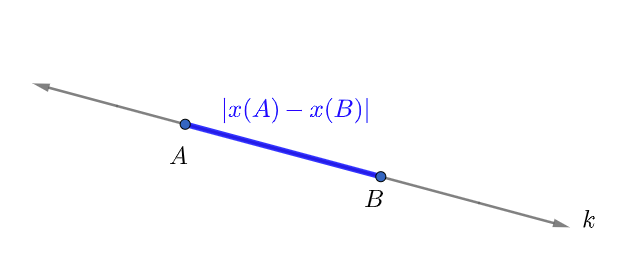
\includegraphics[]{distance.png}
 \end{center}
\end{tcolorbox}
%End Slide  8 xxxxxxxxxxxxxxxxxxxxxxxxxxxxxxxxxxxxxxxxxxxxxxxxxxxxxxxxxxxxxxxxx
\pagebreak

%Slide  9 xxxxxxxxxxxxxxxxxxxxxxxxxxxxxxxxxxxxxxxxxxxxxxxxxxxxxxxxxxxxxxxxxxxx
\marginnote[]{\section{Concept Development}\subsection{Point Plotting Theorem}
\begin{enumerate}
    \item A coordinatization is exactly that ... it is a system for assigning numbers to points and conversely. Emphasize that this is entirely up to the experimenter. But once a coordinatization has been selected, all measurements must be agreed on within that coordinate system. Be very careful if you have to ``change coordinates''. Make sure to keep track of the bookkeeping if you do that. This is especially important in Physics.
    \item Well, we have really only shown ``existence'' ... can you explain why uniqueness also follows? (Answer: If $P'$ is any other point on ray $OQ$ with $\displaystyle{OP'=r,}$ then $\displaystyle{x(P)=x(P')=r}$, and by injectivity of $x$ we have that $\displaystyle{P=P'.}$
    \item Yes! Since $t\mapsto t^2$ is one to one on the positive axis, take $\displaystyle{\zeta = \sqrt{r}}$ and apply the Ruler Postulate. 
\end{enumerate}

}
\begin{tcolorbox}[enhanced jigsaw,breakable,pad at break*=1mm,
  colback=cyan!2!white,colframe=blue!75!black,title=Student View: Slide 9,drop fuzzy shadow,watermark color=white,watermark text=\arabic{tcbbreakpart}]
  \section{Concept Development}\subsection{Point Plotting Theorem}
  From the Ruler Postulate we immediately get the important
  \begin{tcolorbox}[colback=blue!4]
  \textbf{\textit{Point Plotting Theorem:}}
  Let $\overrightarrow{OQ}$ be any given ray. Let $\displaystyle{r>0}$ be given in a specified unit system for measurements on $\overrightarrow{OQ}$ . Then there exists a  unique point $P$ on $\overrightarrow{OQ}$ such that $\displaystyle{OP=r.}$
  
  \end{tcolorbox}
  
  We will be studying the idea of proof very soon. Here we will demonstrate a little bit about what is meant by ``proof''. A proof in mathematics is simply a reasoned arguement based on accepted assumptions. 
  
  \uv What have we to assume here? \textbf{\textit{The Ruler Postulate}}: From this we get a coordinate system ``$x$'' on line $OQ$ with $\displaystyle{x(O)=0}$ and $\displaystyle{x(Q)=1.}$ Hence $\overrightarrow{OQ}$ is the set of points with ``positive'' coordinates in the ``$x$'' system.$^1$
  
  \uv Take $\displaystyle{\zeta = r}$ in the second part of the Ruler Postulate. The postulate assures us the existence of a point $\displaystyle{Z=P}$ with $\displaystyle{x(P)=r}$. Since
  \[OP=|x(P)-x(O)|=|x(P)- 0|=|x(P)|=x(P)=r,
  \]
  we have demonstrated what we desired to show$^2$.
  
  \uv \newthought{Check For Understanding:} Will $x$ composed with  $t\mapsto t^2 $ still give us these results? $^3$ 
  
 
\end{tcolorbox}
%End Slide  9 xxxxxxxxxxxxxxxxxxxxxxxxxxxxxxxxxxxxxxxxxxxxxxxxxxxxxxxxxxxxxxxxx

\pagebreak
%Slide  10 xxxxxxxxxxxxxxxxxxxxxxxxxxxxxxxxxxxxxxxxxxxxxxxxxxxxxxxxxxxxxxxxxxxx
\marginnote[]{\section{Concept Development: Measurement}\subsection{Distance}
\begin{enumerate}
    \item Extended objects are objects which are composed of possibly more than one point. The idea here is to use our notion of distance between points to develop the concept of distance between objects.
    \item In actucality, we should have \[ \text{dist}(\mathcal{T},\mathcal{S})= \inf \{AB \  |  \ A \in \mathcal{T}, B \in \mathcal{S}\}
    \]
    The definition given here works fine when the sets are compact. It is certainly true for simple plane figures like polygons. This is only a course in elementary geometry. So this definition will do well for us. Interested and thoughtful students will do well to consider the shortcomings of this definition. For example, the min does not exist between the point $(2,4)$ and the \textbf{\textit{open}} unit disc. 
\end{enumerate}

}
\begin{tcolorbox}[enhanced jigsaw,breakable,pad at break*=1mm,
  colback=cyan!2!white,colframe=blue!75!black,title=Student View: Slide 10,drop fuzzy shadow,watermark color=white,watermark text=\arabic{tcbbreakpart}]
  \section{Concept Development: Measurement}\subsection{Distance}
\begin{tcolorbox}[colback=blue!4]

\newthought{Knowledge Point:} \textbf{\textit{Distance Between Points}} Let a system of units be selected for measurements of distance between points on ANY line. If $x$ is a coordinate system on line $AB$ then the distance between $A$ and $B$ is $|x(A)-x(B)|.$
\end{tcolorbox}

\uv We define distance between ``extended objects''$^1$ in terms of the distance between points. 

\uv \newthought{Example:} What is the distance between the triangle and the square in the figure below?
\begin{center}
    \scalebox{1}{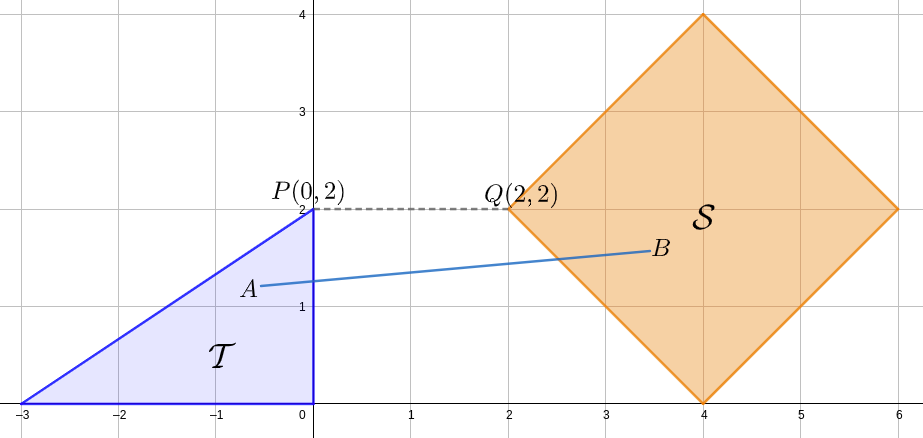
\includegraphics[]{dbtwn1.png}}
\end{center}

Since $\displaystyle{PQ=2}$ and every other segment $\overline{AB}$ with $A$ in $\mathcal{T}$ and $B$ in $\mathcal{S}$ satisfies $\displaystyle{AB>PQ=2}$, we say that the distance between $\mathcal{S}$ and $\mathcal{T}$ is simply $\displaystyle{PQ=2}$. 

\uv\begin{tcolorbox}[colback=blue!4]
\newthought{Definiton:} \textbf{\textit{Distance Between Sets of Points}}

\uv Let $\mathcal{T}$ and $\mathcal{S}$ be sets of points in the plane (or space). We define the \textbf{\textit{distance between }} $T$ and $S$, denoted $\text{dist}(\mathcal{T},\mathcal{S})$ to be the \textbf{\textit{minimum}}$^2$ of all lengths $AB$ where $A$ lies in $\mathcal{T}$ and $B$ lies in $\mathcal{S}.$

\end{tcolorbox}
  
  
 
\end{tcolorbox}
%End Slide 10  xxxxxxxxxxxxxxxxxxxxxxxxxxxxxxxxxxxxxxxxxxxxxxxxxxxxxxxxxxxxxxxx

\pagebreak
%Slide  11 xxxxxxxxxxxxxxxxxxxxxxxxxxxxxxxxxxxxxxxxxxxxxxxxxxxxxxxxxxxxxxxxxxxx
\marginnote[]{\section{Concept Development: Measurement}\subsection{Distance}
\begin{enumerate}
    \item Let $P$ be a point selected off of a given line $k.$ You will want to help the student identify the two sets $\mathcal{T} =\{P\}$ and $\mathcal{S}=k$. The exercise consists in showing that given any arbitrary point $Q$ on $k$ the distance $PQ$ is minimized when $Q$ is on $k^{\perp}(P)\cap k.$ 
    \item This app is very easy to use. Students will see at once that the only way to get the smallest value of $PQ$ is to select that point $Q$ both on $k$ and on the perpendicular $k^{\perp}(P).$
\end{enumerate}

}
\begin{tcolorbox}[enhanced jigsaw,breakable,pad at break*=1mm,
  colback=cyan!2!white,colframe=blue!75!black,title=Student View: Slide 11,drop fuzzy shadow,watermark color=white,watermark text=\arabic{tcbbreakpart}]
 \section{Concept Development: Measurement}\subsection{Distance}
 
 \newthought{Check For Understanding:} Use our generalized definition of \textbf{\textit{Distance Between Sets of Points}} to verify that the right definition of distance from a point to a line is measured along a perpendicular$^1$. 
  
 
\end{tcolorbox}

%End Slide  11 xxxxxxxxxxxxxxxxxxxxxxxxxxxxxxxxxxxxxxxxxxxxxxxxxxxxxxxxxxxxxxxxx
\begin{tcolorbox}[enhanced jigsaw,breakable,pad at break*=1mm,attach boxed title to top center={yshift=-3mm,yshifttext=-1mm},
  colback=yellow!50!white,colframe=yellow,colbacktitle=red!80!black,
  title=Lesson Design Specifications (Please Read),fonttitle=\bfseries,
  boxed title style={size=small,colframe=red!50!black} ]
  \section{Guided Practice: }
 At this point student and teacher will do one of the following: 
    \begin{itemize}
      \item Navigate to Geogebra on a shared screen \textbf{OR}
      \item Launch an app that opens up a shared window for interactive geometry \textbf{OR}
      \item Share a whiteboard with appropriate drawing tools.
  \end{itemize}
  
Here the Instructor will guide the student to use the following app$^2$ which allows the student to move point $Q$ along $k$ and see the distance $PQ$ continuously update. They will see that $PQ$ takes its ``min'' exactly when $Q$ takes on the location of $k^{\perp}(P)\cap k.$ 
\begin{center}
\scalebox{.8}{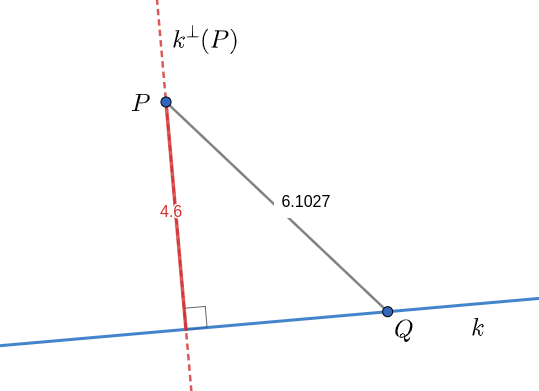
\includegraphics[]{dist2.png}}
\end{center}
\end{tcolorbox}

\pagebreak
%Slide  12 xxxxxxxxxxxxxxxxxxxxxxxxxxxxxxxxxxxxxxxxxxxxxxxxxxxxxxxxxxxxxxxxxxxx
\marginnote[]{\section{Concept Development}\subsection{Symmetry}
\begin{enumerate}
    \item This says that segments formed from images and their pre-images are always perpendicular to the line of reflection.
    \item This says that the line of reflection is fixed under the transformation. 
    \item This says that $k$ contains the midpoints of each of the segments $\overline{R_k(P)P}.$
\end{enumerate}

}
\begin{tcolorbox}[enhanced jigsaw,breakable,pad at break*=1mm,
  colback=cyan!2!white,colframe=blue!75!black,title=Student View: Slide 12,drop fuzzy shadow,watermark color=white,watermark text=\arabic{tcbbreakpart}]
 \section{Concept Development}\subsection{Symmetry}
 \newthought{Definition:} \textbf{\textit{Reflection in a Line:}} Let line $k$ in the plane be given. A \textbf{\textit{reflection}} in $k$ is a function $R_k$ from the plane to itself which has the following properties:
 \begin{enumerate}
     \item For all $P$ not on $k$, $\overline{R_k(P)P}\perp k.$
     \item For all $P$ on $k,$ $R_k(P)=P.$
     \item $k$ is the perpendicular bisector of $\overline{R_k(P)P}$ for all points $P$ not on $k.$ 
 \end{enumerate}
  
 
\end{tcolorbox}
%End Slide  12 xxxxxxxxxxxxxxxxxxxxxxxxxxxxxxxxxxxxxxxxxxxxxxxxxxxxxxxxxxxxxxxxx
\begin{tcolorbox}[enhanced jigsaw,breakable,pad at break*=1mm,attach boxed title to top center={yshift=-3mm,yshifttext=-1mm},
  colback=yellow!50!white,colframe=yellow,colbacktitle=red!80!black,
  title=Lesson Design Specifications (Please Read),fonttitle=\bfseries,
  boxed title style={size=small,colframe=red!50!black} ]
  \section{Guided Practice: }
 At this point student and teacher will do one of the following: 
    \begin{itemize}
      \item Navigate to Geogebra on a shared screen \textbf{OR}
      \item Launch an app that opens up a shared window for interactive geometry \textbf{OR}
      \item Share a whiteboard with appropriate drawing tools.
  \end{itemize}
  
  \uv This sequence of demonstrations will help our students understand the idea of ``reflection in a line'' as a rigid transformation of the plane. This is a huge concept coming up. We get a brief glimpse of it here.
  \pagebreak
  \begin{enumerate}
      \item Reflection of point $P$ in line $k.$
      \begin{center}
          \scalebox{.5}{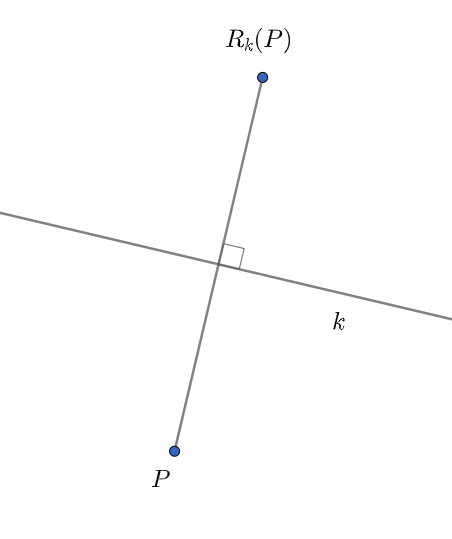
\includegraphics[]{ref1.png}}
      \end{center}
      
      \item Reflection of a segment $PQ$ in line $k.$
      \begin{center}
          \scalebox{.5}{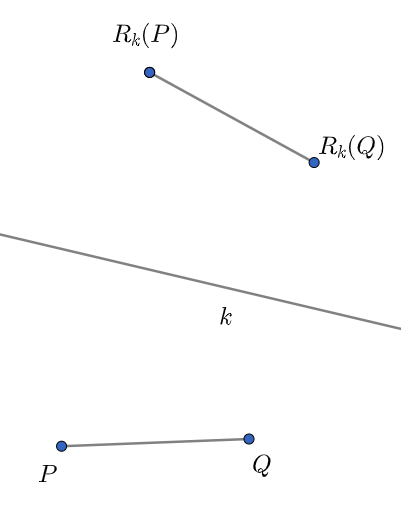
\includegraphics[]{sym2}}
      \end{center}
      
      \pagebreak
      
      \item Reflection of a triangle in line $k.$
      \begin{center}
          \scalebox{.5}{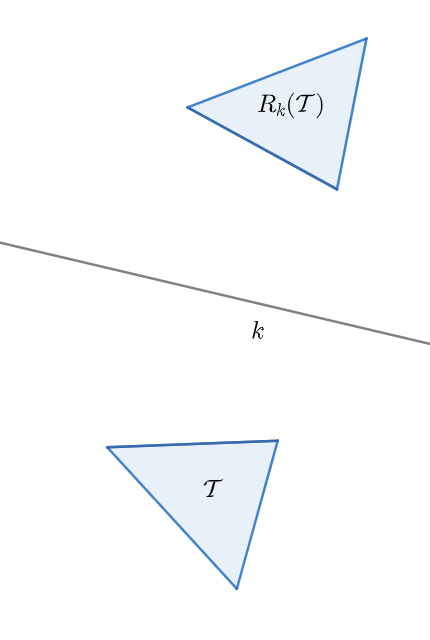
\includegraphics[]{sym3.png}}
      \end{center}
      \item Reflection of a more complicated figure about line $k.$
      \begin{center}
          \scalebox{.5}{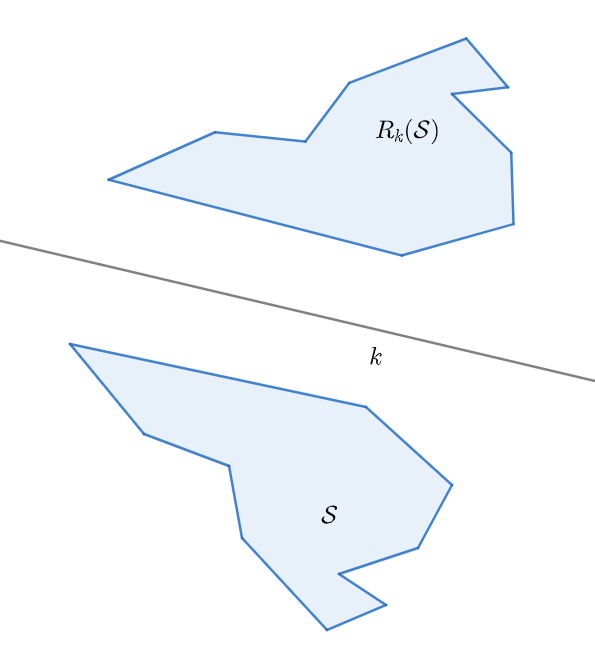
\includegraphics[]{sym4.png}}
      \end{center}
  \end{enumerate}
  We now return to the main instruction sequence.
  \end{tcolorbox} 
  
  \pagebreak
    %Slide  13 xxxxxxxxxxxxxxxxxxxxxxxxxxxxxxxxxxxxxxxxxxxxxxxxxxxxxxxxxxxxxxxxxxxx
\marginnote[]{\section{}\subsection{}
\begin{enumerate}
    \item It cannot be overstated how important this concept is. The idea of symmetry in mathematics is ubiquitous. Later we will investigate rotational symmetry and symmetry via reflection in points. Figures in the plane can be described in large measure by their symmetry groups. For example, a circle is characterized by rotational invariance about its center through every angle, and reflection invariance about every line containing its center. It is also properties of symmetry that inform our ideas of probability; since a coin is ``symmetric'' about its axes of rotation, we should expect a 50:50 chance of getting heads or tails.
    \item It is this fact that allows us to conclude WHY the perpendicular bisectors of the sides of a triangle are concurrent.
    \item It is this fact that allows us to conclude WHY the angle bisectors of a triangle are concurrent.
\end{enumerate}

}
\begin{tcolorbox}[enhanced jigsaw,breakable,pad at break*=1mm,
  colback=cyan!2!white,colframe=blue!75!black,title=Student View: Slide 13,drop fuzzy shadow,watermark color=white,watermark text=\arabic{tcbbreakpart}]
  \newthought{(Huge$^1$) Knowledge Point:} A figure $\mathcal{K}$ is \textbf{\textit{symmetric}} with respect to a line $k$ if $R_k(\mathcal{K})= \mathcal{K.}$
  
  \uvx
  \newthought{Symmetries of Important Figures:} 
  \begin {enumerate}
  
  \item Let $Q$ be a square and let $d$ be a given diagonal. Then $Q$ is symmetric about $d.$
  
  \item Let $d$ be any diameter of any circle. The circle is symmetric about $d.$
  
  
  \item Let $\overline{AB}$ be any given segment. Then $\overline{AB}$  is symmetric with respect to its perpendicular bisector $\mathcal{L}_{AB.}^{\perp}$ $^2$
  
  \item Let angle $\angle ABC$ be given. Let $\overrightarrow{BK}$ be the angle bisector of $\angle ABC.$ Then $\angle ABC$ is symmetric with respect to $\overrightarrow{BK}.$ $^3$
  
  \end{enumerate}
  
 
\end{tcolorbox}
%End Slide  13 xxxxxxxxxxxxxxxxxxxxxxxxxxxxxxxxxxxxxxxxxxxxxxxxxxxxxxxxxxxxxxxxx

\uvx
\begin{tcolorbox}[enhanced jigsaw,breakable,pad at break*=1mm,attach boxed title to top center={yshift=-3mm,yshifttext=-1mm},
  colback=yellow!50!white,colframe=yellow,colbacktitle=red!80!black,
  title=Lesson Design Specifications (Please Read),fonttitle=\bfseries,
  boxed title style={size=small,colframe=red!50!black} ]
  \section{Guided Practice: Demonstrations of Symmetries }
 At this point student and teacher will do one of the following: 
    \begin{itemize}
      \item Navigate to Geogebra on a shared screen \textbf{OR}
      \item Launch an app that opens up a shared window for interactive geometry \textbf{OR}
      \item Share a whiteboard with appropriate drawing tools.
  \end{itemize}
 \uv 1. Use the reflection tool to show that the square is invariant under reflection symmetries in each of the lines $k_x, \ k_y, \ d_x,$ and $d_y.$
 \begin{center}
     \scalebox{1}{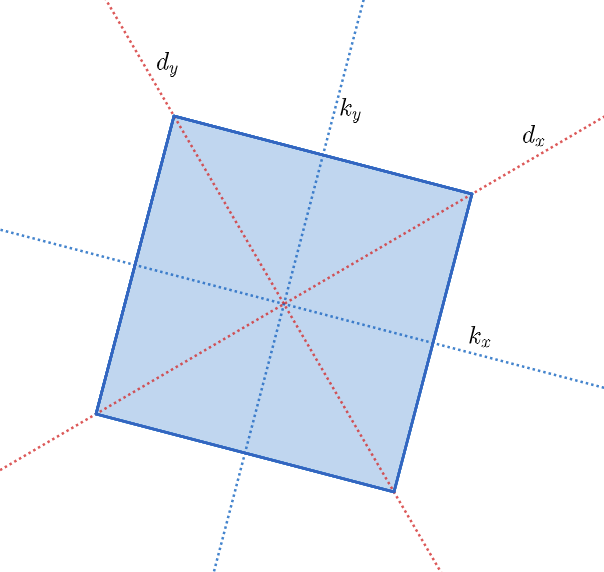
\includegraphics[]{sqref.png}}
 \end{center}
 
 \uvx 2. Use the reflection tool to show that a circle is reflection invariant through any line containing a diameter. Any line $D_Q$ containing the center of a circle $Q$ contains its diameter as shown.
  \begin{center}
     \scalebox{1}{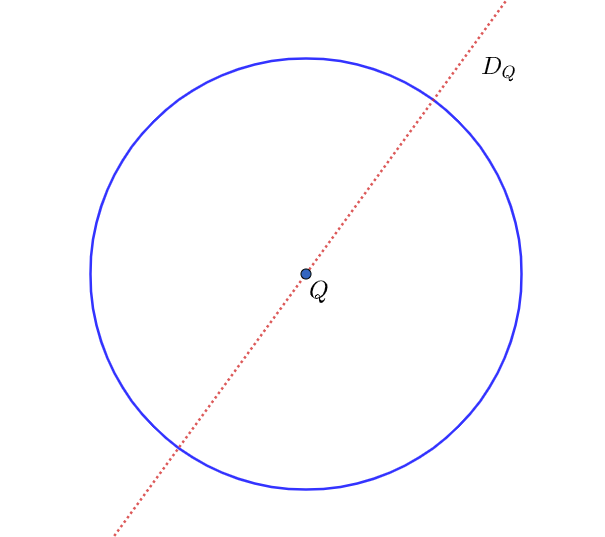
\includegraphics[]{symcir.png}}
 \end{center}
 
 \uvx 3. Use the reflection tool to show that a segment $\overline{AB}$ is reflection invariant about its perpendicular bisector $\mathcal{L}_{AB}^{\perp}$. 
 \begin{center}
     \scalebox{1}{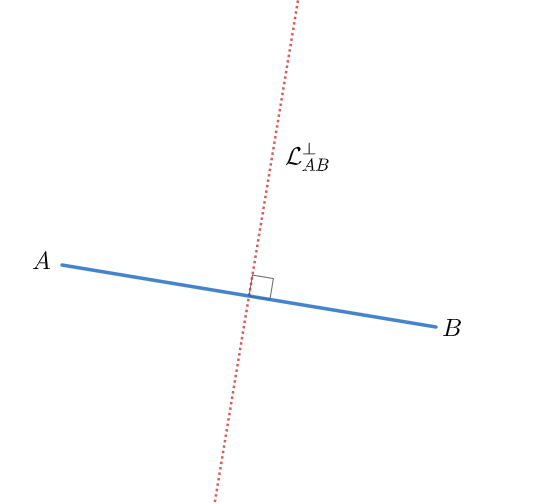
\includegraphics[]{lperp.png}}
 \end{center}


\uvx 4. Use the reflection tool to show that an angle $\angle BAC$ is reflection symmetric about its angle bisector $\overrightarrow{AK}$. 
\begin{center}
     \scalebox{1}{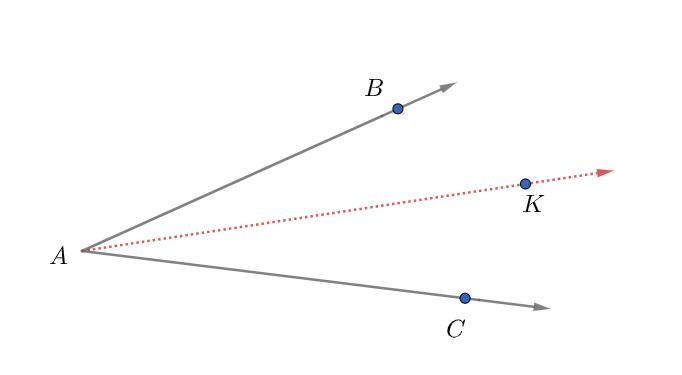
\includegraphics[]{symangle.png}}
 \end{center}
 
 \uvx We now return to the main instruction sequence.
 
 
\end{tcolorbox}
\pagebreak

%Slide  14 xxxxxxxxxxxxxxxxxxxxxxxxxxxxxxxxxxxxxxxxxxxxxxxxxxxxxxxxxxxxxxxxxxxx
\marginnote[]{\section{Application}\subsection{Angle Bisector Theorem}
\begin{enumerate}
    \item It must be emphasized that measurement of distance is along lines perpendicular to the sides of the angle. Any line perpendicular to the angle bisector is is in fact ``bisected'' by it, but that is not the way distance is measured. Make sure to make this point clear. 
    \item If time permits, extend this discussion to account for why the angle bisectors of a triangle must be concurrent. 
\end{enumerate}


}
\begin{tcolorbox}[enhanced jigsaw,breakable,pad at break*=1mm,
  colback=cyan!2!white,colframe=blue!75!black,title=Student View: Slide 14,drop fuzzy shadow,watermark color=white,watermark text=\arabic{tcbbreakpart}]
  
 Let angle $\angle BAC$ be given with angle bisector $\overrightarrow{AK}$. Let $Q$ be any point on $\overrightarrow{AK}$. Then $Q$ is equidistant$^1$ from the sides of $\angle BAC$. 
 
 \uv \newthought{Proof:} Let $m$ be any perpendicular through $\overrightarrow{AK}$ and say $m$ intersects $\angle BAC$ at points $F$ and $G$. Then $\overrightarrow{AK}$ is contained in the perpendicular bisector of $\overline{FG}$ by symmetry. Therefore, given any point on $\overrightarrow{AK}$, say $X$, $\displaystyle{XF=XG}.$ Now take $X$ suitably chosen on ray $AK$ to establish the result.$^2$ 
 
 \uv \begin{center}
     \scalebox{1}{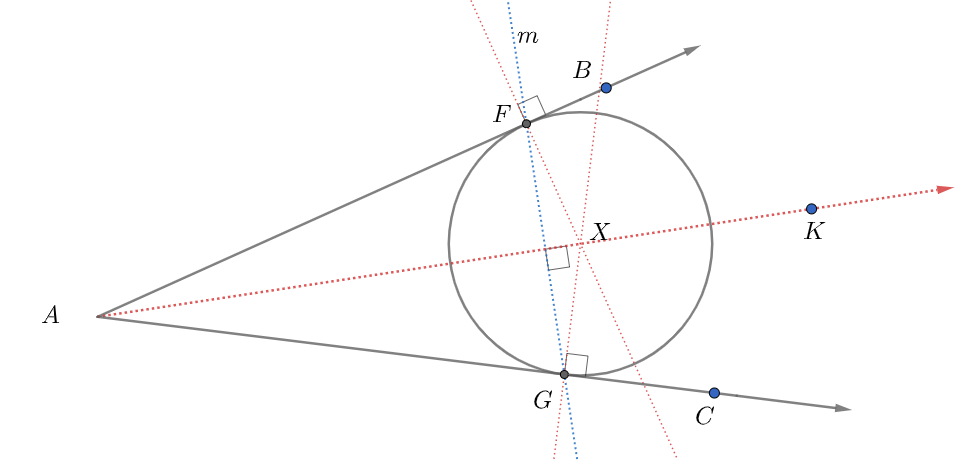
\includegraphics[]{abt.png}}
 \end{center}
 
 
  
 
\end{tcolorbox}
%End Slide   14 xxxxxxxxxxxxxxxxxxxxxxxxxxxxxxxxxxxxxxxxxxxxxxxxxxxxxxxxxxxxxxxxx
 \pagebreak
 
 %Slide  15 xxxxxxxxxxxxxxxxxxxxxxxxxxxxxxxxxxxxxxxxxxxxxxxxxxxxxxxxxxxxxxxxxxxx
\marginnote[]{\section{Applications}\subsection{Explaining Concurrencies}
\begin{enumerate}
    \item In this first discussion, note that the distances are computed from the circumcenter to the vertices of the triangle. Since the bisectors of the sides of the triangle are lines of symmetry, their incidence point forms three isosceles triangles with respect to the vertices of the ambient figure. This is the heart of the reasoning here.
    \item In the second discussion the emphasis is on the distance between the alleged point of concurrence and the the sides of the angles. Note that in both discussions, critical dependence is made on the concept of measure. In both of these discussions we are preparing students to be able to fashion arguments for themselves using reasoning skills based on previously established facts and assumed principles.
    
\end{enumerate}

}
\begin{tcolorbox}[enhanced jigsaw,breakable,pad at break*=1mm,
  colback=cyan!2!white,colframe=blue!75!black,title=Student View: Slide 15,drop fuzzy shadow,watermark color=white,watermark text=\arabic{tcbbreakpart}]
 \newthought{Check For Understanding:} How does the concept of symmetry help us understand WHY:
 \begin{enumerate}
     \item The perpendicular bisectors of the sides of a triangle are concurrent.
     \item The angle bisectors of the angles of a triangle are concurrent.
 \end{enumerate}
 
 \uv \newthought{Explanation of 1.}
 \uv \begin{center}
     \scalebox{.8}{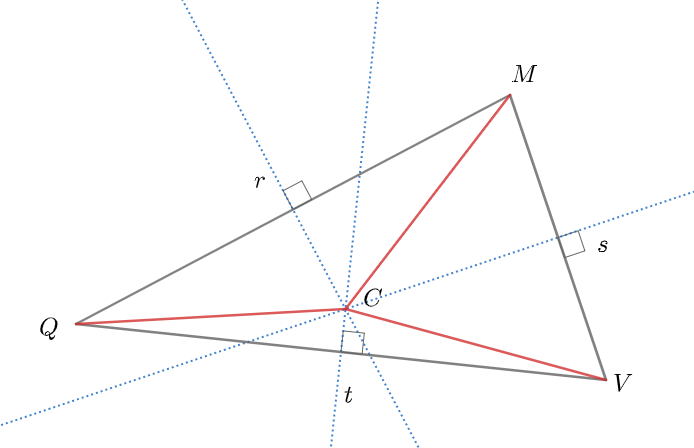
\includegraphics[]{circent.png}}
 \end{center}
  
  \uv \newthought{Given} $\triangle QMV$ with circumcenter $C$ on lines $r, s$ as shown. We need to explain WHY $C$ also lies on $t.$ Here is why. $r$ is the perpendicular bisector of segment $QM$ and C is on the intersection of $r$ and $s$. Therefore $\displaystyle{CQ=CM}.$ But $C$ is also on $s,$ the perpendicular bisector of segment $MV,$ hence $\displaystyle{CM=CV}$ and it follows therefore that $\displaystyle{CQ=CV}$ since these are both equal to $CM.$ Since $CQ=CV,$ it follows that $C$ must be equidistant from $Q$ and $V$ which means that $C$ is on $t,$ the perpendicular bisector of $\overline{QV}$. It follows that $r,s,t$ must be concurrent at $C.$
  
  \pagebreak
  \newthought{Explanation of 2.}
  
  
 \uv \begin{center}
     \scalebox{.8}{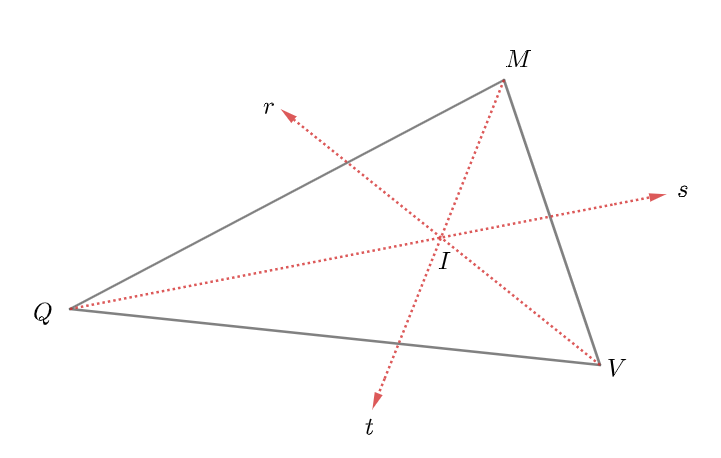
\includegraphics[]{incentproof.png}}
 \end{center}
 
 \uv \newthought{Given} $\triangle QMV$ with incenter $I$ on angle bisectors $r, s$ as shown. We need to explain WHY $I$ also lies on angle bisector $t.$ Here is why. Since $I$ lies on the angle bisector $r,$ \[ \text{dist}(I, \overline{MV})=\text{dist}(I,\overline{QV}).\] Now, since $I$ also lies on the angle bisector $s,$ \[ \text{dist}(I, \overline{QM})=\text{dist}(I,\overline{QV}).\] Hence \[ \text{dist}(I, \overline{QM})=\text{dist}(I,\overline{MV}).\] And this means that $I$ must lie on the angle bisector of $\angle QMV$ which of course is $t.$ 
 
\end{tcolorbox}
%End Slide 15  xxxxxxxxxxxxxxxxxxxxxxxxxxxxxxxxxxxxxxxxxxxxxxxxxxxxxxxxxxxxxxxxx

\pagebreak

 %Slide 16  xxxxxxxxxxxxxxxxxxxxxxxxxxxxxxxxxxxxxxxxxxxxxxxxxxxxxxxxxxxxxxxxxxxx
\marginnote[]{\section{Concluding Thoughts}\subsection{}


}
\begin{tcolorbox}[enhanced jigsaw,breakable,pad at break*=1mm,
  colback=cyan!2!white,colframe=blue!75!black,title=Student View: Slide 16,drop fuzzy shadow,watermark color=white,watermark text=\arabic{tcbbreakpart}]
We have done what we set out to do. \dCooley[-3][yellow]  

\uv In this lesson we have covered a lot of material!
\begin{itemize}
    \item We reviewed our basic constructions and learned more about constructiong perpendicular and parallel lines.
    \item We introduced the formal term ``postulate'' that we will continue to use throughout this course.
    \item We discussed in detail the meaning of measurement.
    \item We introduced the concept of symmetry and its role in geometry.
    \item We concluded with clear explanations of why the concurrencies we saw in lessons 4 and 5 must be the case.
\end{itemize}

In our next lesson we will continue to apply these ideas and discuss further conclusions we can draw regarding angles, lines and structures associated with them. 
  
 
\end{tcolorbox}
%End Slide  16 xxxxxxxxxxxxxxxxxxxxxxxxxxxxxxxxxxxxxxxxxxxxxxxxxxxxxxxxxxxxxxxxx 
  
  

 
 
 


 




\end{document}